\chapter{Sistemas No Lineales}
Consideramos en este capítulo sistemas planos autónomos $\dot{x} = f(x)$ donde $f$ es una función no necesariamente lineal en $x = (x_1,x_2)$.

Supondremos $f$ de al menos clase $C^1$ de manera que sea posible considerar la linealización de $f$ mediante su derivada (matriz jacobiana) y estudiar las propiedades de este sistema lineal con el objetivo de deducir información sobre el comportamiento del sistema original.

A continuación formalizamos el concepto de linealización mediante expansión en serie de Taylor (sección \ref{sec:linealizacion}).

\section{Linealización} \label{sec:linealizacion}

Consideremos un sistema plano como en la ecuación \ref{eq:sistema_dinamico_plano_v0}, de la forma

\begin{equation}
	\dot{x} = f(x) = (f_1(x_1,x_2), f_2(x_1,x_2)),
\end{equation}

donde $f$ es una función arbitraria de clase $C^1$.

En este caso no necesariamente el sistema tiene un punto crítico en $x = 0$ y mucho menos debe ser el único.

\begin{example}Como vimos en el ejemplo \ref{ej:pendulo}, el péndulo matemático está descrito por la ecuación diferencial de segundo orden $\ddot{x} + \sin(x) = 0$ que puede escribirse en forma vectorial con $x = (x_1,x_2)$ como

$$
\begin{array}{lll}
	\dot{x_1} & = & x_2 \\
	\dot{x_2} & = & -\sin(x_1).
\end{array}
$$

Por lo tanto el péndulo matemático tiene un punto crítico en $(x_1,x_2) = (0,0)$ pero también en todos los puntos $(n\pi, 0)$ para $n \in \Z$.
\end{example}

Supongamos entonces que $x^1, x^2, ..., x^n, ...$ son puntos críticos del sistema $\dot{x} = f(x)$ y que son aislados (es decir, existe una vecindad  $V_i$ de $x^i$ donde $x^i$ es el único punto crítico).

Sea $\bar{x}$ uno de estos puntos críticos y supongamos que $f$ es diferenciable en $\bar{x}$. Entonces podemos expandir $f$ como serie de Taylor alrededor de $f$ y escribir para $x$ cerca de $\bar{x}$:

\begin{equation} \label{eq:expansiontaylor1}
	f(x) = f(\bar{x}) + Df(\bar{x})(x - \bar{x}) + h(x)
\end{equation}

donde $|| \frac{h(x)}{x - \bar{x}}|| \to 0$ cuando $x \to \bar{x}$.

Ahora, como $\bar{x}$ es un punto crítico entonces $f(\bar{x}) = 0$ y la fórmula \ref{eq:expansiontaylor1} se reduce a 

\begin{equation}
	f(x) = Df(\bar{x})(x - \bar{x}) + h(x).
\end{equation}

Por lo tanto, el sistema no lineal, cerca de $\bar{x}$ es

$$ \dot{x} = f(x) = Df(\bar{x})(x - \bar{x}) + h(x).$$

Si a continuación introducimos el cambio de coordenadas $y = x - \bar{x}$ entonces tenemos 

\begin{equation} \label{eq:cuasilineal}
	\dot{y} = Df(\bar{x})y + g(y).
\end{equation}

En la ecuación \ref{eq:cuasilineal}, $g(0) = 0$ y $Dg(0) = 0$ así que el Teorema del Valor Medio implica que $g(y)$ es ``pequeño'' en comparación a $y$ cerca del origen. Más precisamente, dado $m > 0$ existe $\delta > 0$ tal que 

$$ ||g(y)|| \leq m||y||$$

siempre que $||y|| < \delta$.

En otras palabras, $g(y)$ puede hacerse tan pequeño como se desee tomando $y$ suficientemente pequeño. Por esta razón resulta natural pensar que la estabilidad de $\bar{x}$ pueda describirse en términos del sistema lineal

\begin{equation} \label{eq:linealizacion}
	\dot{y} = Df(\bar{x})y.
\end{equation}

Si $Df(\bar{x})$ es invertible, el único punto crítico es $\bar{y} = 0$ y puede clasificarse según los criterios vistos en la sección \ref{sec:estabilidadlineal}.
Se quisiera poder llegar a las mismas conclusiones para $\bar{x}$, pero esto no será siempre posible como se verá más adelante.

\section{Criterio de estabilidad para sistemas no lineales}
A partir de la linealización de $f$ en un punto crítico $\bar{x}$ es posible a veces determinar la estabilidad del mismo de manera análoga al caso lineal (teorema \ref{teo:criterioestabilidadlineales}).

El siguiente teorema, cuya prueba puede encontrarse en \cite[p.~267,272]{dynandbif}, describe la estabilidad en dos casos particulares.

\begin{theorem}[Criterio de estabilidad para sistemas no lineales] \label{teo:criterioestabilidadnolineales}
Sea $f$ de clase $C^1$, $\dot{x} = f(x)$ un sistema plano y $\bar{x}$ un punto crítico del mismo.

\begin{enumerate}[(a)]
	\item Si todos los valores propios de $Df(\bar{x})$ tienen parte real negativa, entonces $\bar{x}$ es un punto crítico asintóticamente estable (y por lo tanto, estable).
	\item Si al menos un valor propio de $Df(\bar{x})$ tiene parte real positiva entones $\bar{x}$ es un punto crítico inestable.
\end{enumerate}
\end{theorem}

\begin{example} \label{ex:nolinealhiperbolico}
Considérese el sistema no lineal

$$ \begin{array}{l} \dot{x_1} = x_1^2 + x_2^2 - 6 \\ \dot{x_2} = x_1^2 - x_2 \end{array}. $$

Los puntos críticos son $(\sqrt{2}, 2)$ y $(-\sqrt{2}, 2)$ y la matriz jacobiana $Df(x)$ está dada por

$$ Df(x) = \left( \begin{array}{ll} 2x_1 & 2x_2 \\ 2x_1 & -1 \end{array} \right).$$

Sean

$$
	A_1 = Df((\sqrt{2},2)) = \left(\begin{array}{ll} 2\sqrt{2} & 4 \\ 2\sqrt{2} & -1 \end{array} \right), \hspace{8pt}
	A_2 = Df((-\sqrt{2},2)) = \left(\begin{array}{ll} -2\sqrt{2} & 4 \\ -2\sqrt{2} & -1 \end{array} \right).	
$$

$A_1$ tiene un valor propio real positivo pues $\det(A_1) < 0$ así que puede concluirse que $(\sqrt{2}, 2)$ es un punto crítico inestable.
Por otro lado, $A_2$ tiene determinante positivo y traza negativa, así que ambos valores propios tienen partes reales negativas. Por el criterio de estabilidad, $(-\sqrt{2},2)$ es un punto crítico estable.

Aunque aún no podemos asegurarlo (más adelante se hará) podríamos pensar que el punto crítico $(-\sqrt{2}, 2)$ es un punto de espiral. Este sería el caso si el sistema fuera lineal y, como ilustra la figura \ref{fig:nolinealhiperbolico-espiral}, la evidencia numérica refuerza esta idea.

\begin{figure} \centering
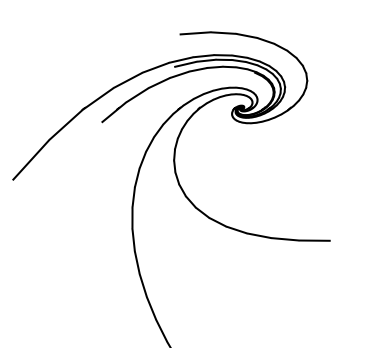
\includegraphics[scale=0.45]{figures/nolinealhiperbolico-espiral.png}
\caption{$\clubsuit$ Diagrama de fase en cercanías del punto crítico $(-\sqrt{2}, 2)$.}
\label{fig:nolinealhiperbolico-espiral}
\end{figure}

\end{example}

Nótese que el teorema \ref{teo:criterioestabilidadnolineales} no ofrece información alguna para cuando hay valores propios con parte real nula. Esto no es casualidad pues en tal caso no es posible determinar la naturaleza del punto crítico a partir de la linealización, como ilustra el siguiente ejemplo.

\begin{example} \label{ex:nolinealnohiperbolico}
Sea $\mu \in \R$ arbitrario y consideremos el sistema no lineal

$$
	\begin{array}{l}
		\dot{x_1} = x_2 + \mu x_1(x_1^2 + x_2^2) \\
		\dot{x_2} = x_1 + \mu x_2(x_1^2 + x_2^2).
	\end{array}
$$

La linealizacíon del sistema en el punto crítico $\bar{x} = 0$ es $\dot{x} = Df(\bar{x})x = \left( \begin{array}{ll} 0 & 1 \\ -1 & 0 \end{array} \right) x,$ sin importar el valor de $\mu$.
Los valores propios de $Df(\bar{x})$ son $\lambda_{1,2} = \pm i$, de manera que no podemos utilizar el criterio de estabilidad pues tienen parte real nula. La razón la ofrece el siguiente argumento.

Notemos que

$$ \dfrac{d}{dt} (x_1^2 + x_2^2) = 2\mu(x_1^2 + x_2^2)^2. $$

Entonces, si $\mu < 0$, $||x(t)|| \to 0$ cuando $t \to \infty$ y por lo tanto $\bar{x} = 0$ es asintóticamente estable.
Si en cambio $\mu > 0$ entonces $||x(t)|| \to \infty$ cuando $t \to \infty$ y el punto crítico $\bar{x} = 0$ resulta ser inestable.

Esta dependencia de $\mu$ no aparece en la linealización del sistema y por lo tanto este ejemplo demuestra que el teorema \ref{teo:criterioestabilidadnolineales} es tan preciso como es posible.
\end{example}


\section{Clasificación de puntos críticos}

Quisiéramos repetir la clasificación hecha en la sección \ref{sec:estabilidadlineal} para los puntos críticos de sistemas no lineales y nombrar los puntos críticos como nodos, puntos de silla, centros, etc.

Por supuesto, la idea es utilizar la linealización para tal fin, sin que sea necesario resolver el sistema de manera explícita.

Desde el principio sabemos que esta tarea no es tan sencilla como en el caso lineal: el ejemplo \ref{ex:nolinealnohiperbolico} demuestra que cuando hay valores propios con parte real nula no podemos ni siquiera determinar utilizando solo la matriz jacobiana la estabilidad del punto crítico, mucho menos deducir si se trata de un centro, punto espiral, nodo, etc.

Por el contrario, si se vuelve al diagrama de fase del ejemplo \ref{ex:nolinealhiperbolico} notamos que no sólo pudimos deducir, utilizando el criterio de estabilidad, la estabilidad de los puntos críticos sino que estos coinciden, además con el tipo de punto crítico del sistema linealizado. Por ejemplo, para $\bar{x} = (-\sqrt{2},2)$ el sistema lineal tiene un punto de espiral y este es el mismo comportamiento que presenta el punto crítico en el sistema no lineal.

Podría pensarse, entonces, que las dificultades aparecen únicamente cuando la matriz jacobiana $Df(\bar{x})$ no es hiperbólica, es decir, tiene valores propios con parte real nula y que, en caso contrario, las soluciones del sistema no lineal tienen el mismo comportamiento geométrico que las del sistema lineal correspondiente. En efecto, este es el caso, como se verá a continuación.

\subsection{Puntos críticos hiperbólicos}

\begin{definition}Un punto crítico $\bar{x}$ de un sistema plano $\dot{x} = f(x)$ es \emph{hiperbólico} si la matriz jacobiana en ese punto, $Df(\bar{x})$ es hiperbólica (tiene valores propios todos con parte real no nula).
\end{definition}

Ya sabemos del ejemplo \ref{ex:nolinealnohiperbolico} que en puntos críticos no hiperbólicos puede ser imposible conocer el comportamiento de las soluciones en vecindad del mismo a partir de la linealización. El caso es contrario cuando se trata de puntos hiperbólicos, como demuestra el siguiente teorema.

\begin{theorem}[Hartman-Grobman] \label{teo:hartmangrobman}
Sea $f$ de clase $C^1$ y $\bar{x}$ un punto crítico \emph{hiperbólico} del sistema plano $\dot{x} = f(x)$. Entonces hay una vecindad de $\bar{x}$ en la cual $\dot{x} = f(x)$ es topológicamente equivalente a su linealización $\dot{x} = Df(\bar{x})x$.
\begin{proof}
Ver \cite[p.~136]{barrvalls}.
\end{proof}
\end{theorem}

El teorema anterior garantiza, entonces, que para puntos críticos hiperbólicos el comportamiento del sistema no lineal cerca del punto es ``idéntico'' al del sistema lineal correspondiente y por tanto todas las nociones antes vistan coinciden.

Para puntos críticos no hiperbólicos es necesario utilizar otras técnicas (o hallar las soluciones del sistema) para determinar el comportamiento.

Combinando el teorema \ref{teo:hartmangrobman} con el criterio de estabilidad (teorema \ref{teo:criterioestabilidadnolineales}) es posible construir la tabla \ref{tab:clasificacionequilibrios}, que clasifica los equilibrios de sistemas no lineales (por supuesto, también aplica para lineales).

\begin{table}[ht!]
{\small
	\begin{tabular}{|c|c|c|c|c|}
		\hline
		\textbf{Vlrs propios de $Df(\bar{x})$} & \multicolumn{2}{|c|}{\textbf{Linealización}} & \multicolumn{2}{|c|}{\textbf{Sistema no lineal}} \\
		\hline
		 & \textbf{Tipo} &\textbf{Estabilidad} & \textbf{Tipo} & \textbf{Estabilidad} \\
		\hline
		\multicolumn{5}{|c|}{\textit{Equilibrios Hiperbólicos}} \\
		\hline
		$\lambda_1 > \lambda_2 > 0$ & nodo & inestable & nodo & inestable \\
		$\lambda_1 < \lambda_2 < 0$ & nodo & A. E. & nodo & A. E. \\
		$\lambda_2 < 0 < \lambda_1$ & punto silla & inestable & punto silla & inestable \\
		$\lambda_{1,2} = a \pm ib, a > 0$ & punto espiral & inestable & punto espiral & inestable \\
		$\lambda_{1,2} = a \pm ib, a < 0$ & punto espiral & A. E. & punto espiral & A. E. \\

		\hline
		\multicolumn{5}{|c|}{\textit{Equilibrios no Hiperbólicos}} \\
		\hline
		$\lambda_1 = \lambda_2 >0$ & nodo propio o impropio & inestable & nodo o punto espiral & inestable \\
		$\lambda_1 = \lambda_2 < 0$ & nodo propio o impropio & A. E. & nodo o punto espiral & A. E. \\
		$\lambda_{1,2} = \pm ib$ & centro & estable & centro o punto espiral & \textbf{?} \\
		\hline
	\end{tabular}
}
	\label{tab:clasificacionequilibrios}
	\caption{Clasificación de equilibrios en sistemas no lineales.}
\end{table}
